\subsection{(Property-Based) Testing as a Semi-Formal Method}

\begin{frame}
\frametitle{(Property-Based) Testing as a Semi-Formal Method}

\begin{quote}
    ``\textit{Program testing can be a very effective way to show the presence of bugs, but it is hopelessly inadequate for
    showing their absence''}\cite{humbleprogrammer1972}
    \begin{flushright}
    --- Edsger W. Dijkstra, The Humble Programmer (1972)
    \end{flushright}
\end{quote}

\end{frame}

\begin{frame}[fragile]
\frametitle{(Property-Based) Testing as a Semi-Formal Method}
\begin{verbatim}
    for all inputs x, y, ...
    such that precondition(x, y, ...) holds,
    P(x, y, ...) is true
\end{verbatim}
\begin{itemize}
    \item \coqcode{P} is a mathematical property
    \item Inputs \coqcode{x, y, ...} are generated \textit{arbitrarily} (using some generative func)
    \item Potentially thousands of test cases are generated \& executed
\end{itemize}


\end{frame}

\begin{frame}
\frametitle{PBT versus other testing methods}
\begin{figure}
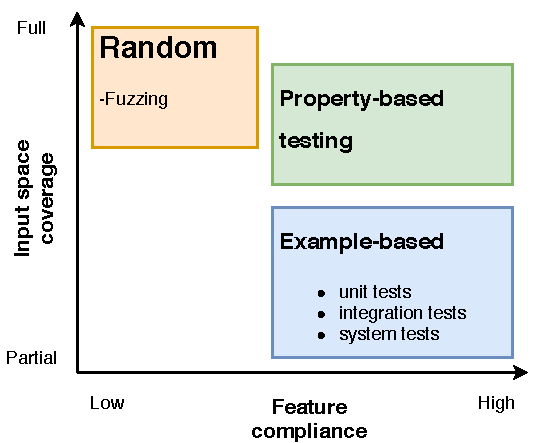
\includegraphics[scale=0.7]{media/Testing-diagram.pdf}
\end{figure}
\end{frame}

% \begin{splitframe}{0.33}{0.72}{PBT Automation vs. Performance vs. Effectiveness}
% {
% \begin{itemize}
%     \item Sometimes ``random'' data is not sufficient
%     \item Trade-off: automation vs. performance
%     \item Specialized generators $\Rightarrow$ less coverage
%     \item The right approach? Depends on the use-case...
% \end{itemize}
% }
% {
% \begin{figure}
% 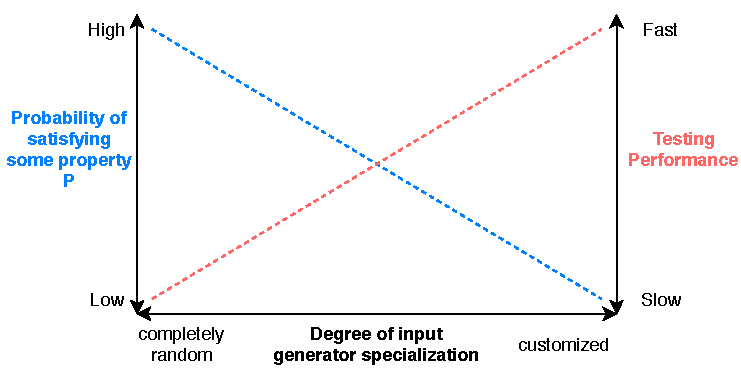
\includegraphics[scale=0.65]{media/random-vs-specialized-generators.pdf}
% \end{figure}
% }
% \end{splitframe}

\section{Contributions}
\begin{frame}{Contributions}
\begin{itemize}
    \item A PBT framework for ConCert smart contracts in Coq
    \item Functional and temporal properties on automatically generated execution traces
    \item Several case studies of complex contracts
    \begin{itemize}
        \item ERC20 Tokens, Congress, FA2 Tokens, UniSwap token exchange
        \item Successfully tested many safety properties on these
        \item Discovered known re-entrancy bugs and other vulnerabilities using testing
    \end{itemize}
\end{itemize}
\end{frame}

\section{A Brief Introduction to ConCert}
\begin{frame}
\frametitle{A Brief Introduction to ConCert}
\begin{itemize}
    \item Blockchain \& Smart Contract formalisation in Coq
    \item Certified extraction to Liquidity and Midlang
    \item Contains a certified, \textit{executable} execution framework
    \item Functional contracts as Coq terms
    \item Contracts consist of an \coqcode{init} and \coqcode{receive} function
\end{itemize}
\end{frame}

\defverbatim[colored]\initfun{
\begin{coq}
Parameter (State Msg Setup : Type).
init :
  Chain ->
  ContractCallContext ->
  Setup ->
  option State;
\end{coq}
}

\defverbatim[colored]\receivefun{
\begin{coq}
Parameter (State Msg Setup : Type).
receive :
  Chain ->
  ContractCallContext ->
  State ->
  option Msg ->
  option (State * list ActionBody);
\end{coq}
}


\begin{frame}{A Brief Introduction to ConCert}{Contract Representation}
\initfun
\end{frame}

\begin{frame}{A Brief Introduction to ConCert}{Contract Representation}
\receivefun
\end{frame}

\begin{frame}{A Brief Introduction to ConCert}{Execution Model}
\begin{itemize}
    \item Each block holds the states of all deployed contracts
    \item and a list of \coqcode{Action}s to execute in this block
    \item \coqcode{Action}s can be: contract calls, transfers, contract deployments
    \item Execution trace: a sequence of blocks where no actions failed 
\end{itemize}
\end{frame}

\section{A Motivating Example: ERC20 Tokens}

\begin{frame}{A Motivating Example: ERC20 Tokens}
\begin{itemize}
    \item Tokens can represent any asset
    \item Transferable
    \item Widely used and backbone of many smart contracts
    \item ERC20: \coqcode{transfer, transfer\_from, approve}
\end{itemize}
\end{frame}


\defverbatim[colored]\ercmsg{
\begin{coq}
Inductive Msg :=
| transfer : Address -> N -> Msg
| transfer_from : Address -> Address -> N -> Msg
| approve : Address -> N -> Msg.
\end{coq}
}

\defverbatim[colored]\ercreceive{
\begin{coq}
Definition receive chain ctx state maybe_msg :=
  ...
  match maybe_msg with
  | Some (transfer to amount) => try_transfer ...
  | Some (transfer_from from to amount) => try_transfer_from ...
  | Some (approve delegate amount) => try_approve ...
  | None => None
  end.
\end{coq}
}

\defverbatim[colored]\ercstate{
\begin{coq}
Record State := {
  total_supply : N;
  balances : FMap Address N;
  allowances : FMap Address (FMap Address N)
}.
\end{coq}
}

\begin{frame}{A Motivating Example: ERC20 Tokens}{ConCert Contract Implementation}
\ercmsg
\ercstate
\end{frame}


\begin{frame}{A Motivating Example: ERC20 Tokens}{ConCert Contract Implementation}
\ercreceive
\end{frame}

\begin{frame}{A Motivating Example: ERC20 Tokens}{Specification}
What is the specification of ERC20?
\begin{itemize}
    \item \coqcode{transfer} updates balances correctly
    \item \coqcode{transfer\_from} updates balances correctly, and access control is applied correctly
    \item \coqcode{approve} updates the allowances correctly
\end{itemize}
Can easily be stated as functional properties, and either tested or proved. All is good, then? Not quite...
\end{frame}

\begin{frame}{A Motivating Example: ERC20 Tokens}{A Vulnerability}
Attack on \coqcode{approve+transfer\_from}:
\begin{enumerate}
    \item Alice approves Bob for $N$ tokens
    \item Alice re-approves Bob for $M$ ($M < N$) tokens
    \item Bob notices this and transfers $N$ of Alices tokens somewhere
    \item if Bob's transaction is executed \textit{before} Alice's, then he can now transfer another $M$ tokens.
\end{enumerate}
\begin{itemize}
    \item Thus, Bob can transfer up to $N + M$ tokens, while Alice expected at most $M$ tokens.
    \item \textbf{All ERC20 compliant tokens are vulnerable to this (in Ethereum)}
\end{itemize}
\end{frame}

\begin{frame}{A Motivating Example: ERC20 Tokens}{Safety Property Guarding against the Attack}
\begin{itemize}
    \item What is the safety property?
    \item Must necessarily be defined over an entire \textit{execution trace} \item Should be able to compare state of ERC20 contract at different steps in execution trace
\end{itemize}
\end{frame}

\begin{frame}{A Motivating Example: ERC20 Tokens}{Safety Property Guarding against the Attack}
In ``verbatim'':
\begin{itemize}
    \item Let $S$, $S'$ be ERC20 contract states.
    \item If $S$ is the result of an \coqcode{approve} act $P$ for $N$ tokens,
    \item and if $S'$ is the result of the same \coqcode{approve} act but with $M$ tokens,
    \item if $S \rightsquigarrow S'$
    \item then the delegate has transferred $\le N$ tokens from the owner in this interval
\end{itemize}
\textbf{I have stated and tested this property (QC finds a counterexample just like the attack)}\\
Next: How the testing framework supports this
\end{frame}